\section{掛金}

% 1節 事業主掛金
\subsubsection{事業主掛金の年単位化}
\barquo{
  以下のBさんについて、(a)、(b)それぞれにおける金額を入力しなさい。なお、算出
  過程についても入力すること。 ((a)、(b)それぞれ100 字以内)

  \;

  <Bさんの情報>
  \begin{itemize}
    \item 企業型年金に加入しており、確定拠出年金法施行令に規定する他制度加入者、個人型年金同時加入可能者のいずれにも該当しない
    \item 企業型年金加入者掛金の拠出はない
    \item Bさんが加入している企業型年金の拠出区分期間は3か月(年4回(3月、6月、9月、12月)の各月に前月までの分の事業主掛金を拠出)である
  \end{itemize}
  
  \begin{enumerate}
    \renewcommand{\labelenumi}{(\alph{enumi})}
    \item 2022 年(令和4 年)12 月に60,000 円(月額ベースで20,000 円)、2023 年(令和5 年)
      3 月に60,000 円(月額ベースで20,000 円)の事業主掛金を拠出した場合の2023 年(令和
      5 年)6 月における事業主掛金の最大額
    \item 2023 年(令和5 年)3 月に60,000 円(月額ベースで20,000 円)、2023 年(令和5 年)6
      月に60,000 円(月額ベースで20,000 円)、2023 年(令和5 年)9 月に80,000 円(月額ベ
      ース20,000 円に加え賞与のあった6 月分は20,000 円を加算)の事業主掛金を拠出した場
      合の2023 年(令和5 年)12 月における事業主掛金の最大額
  \end{enumerate}

  \rightline{引用元:年金1 2023 問2(2)(ウ) }
}

\begin{itembox}[l]{\textgt{ポイント}}
  法第19条。
  2018年1月1日施行で、事業主掛金を\textcolor{red}{年単位}で拠出することが可能になった。

  \;

  \begin{center}
    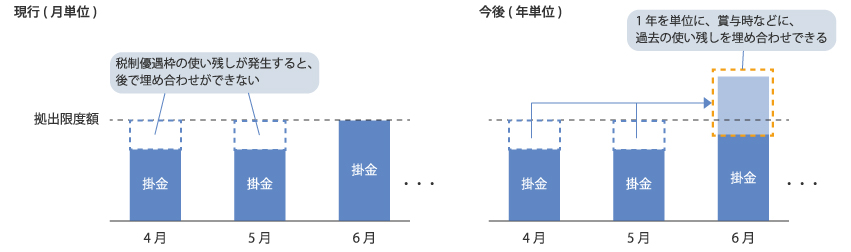
\includegraphics[width=130mm]{figure/nentanika.jpg}
  \end{center}

  \rightline{図の引用元:\url{https://kumitateru.jp/media/topic/a46} }

  
  年単位化により比較的自由に事業主掛金を拠出できるようになったが、以下のようなルールが存在する。

  \begin{itemize}
    \item その月までの拠出限度額を超えてはいけない(令第11条の2)
    \item 拠出区分期間の変更は年1回まで(解釈第1-2.(7))
  \end{itemize}
  
\end{itembox}

\begin{sol}
  \;

  \begin{enumerate}
    \renewcommand{\labelenumi}{(\alph{enumi})}
    \item 2023年6月時点で拠出可能な事業主掛金の総額は、$55,000(円) \times 6(月) = 330,000(円)$。
    
    2023年6月時点で実際に拠出している事業主掛金は、2023年3月拠出の$60,000$(円)。

    したがって、2023年6月に拠出できる事業主掛金の最大額は、$330,000(円)- 60,000(円)=\textcolor{red}{270,000(円)}$。
    
    \item 2023年12月時点で拠出可能な事業主掛金の総額は、$55,000(円) \times 12(月) = 660,000(円)$。

    2023年12月時点で実際に拠出している事業主掛金は、2023年3、6、9月に拠出した事業主掛金の合計額なので、
    $60,000(円)+60,000(円)+80,000(円) = 200,000(円)$。

    したがって、2023年12月に拠出できる事業主掛金の最大額は、$660,000(円)-200,000(円)=\textcolor{red}{460,000(円)}$。

  \end{enumerate}
\end{sol}

\newpage

\subsubsection{事業主掛金の算定方法:不当に差別的なもの}
\barquo{
  確定拠出年金法施行令第6 条第2 号において、事業主掛金の額の算定方法等は、特定の者に
  ついて不当に差別的なものでないこととされている。また、同条第4 号において、企業型年
  金加入者が掛金を拠出することができることを企業型年金規約に定める場合の要件が定めら
  れており、企業型年金加入者掛金の額の決定又は変更の方法は、特定の者について不当に差
  別的なものでないこととされている。

  この「不当に差別的なものでないこと」に該当しないものとして『確定拠出年金法並びにこ
  れに基づく政令及び省令について(法令解釈)』に例示されているものを2 つ簡潔に入力しな
  さい。

  \rightline{引用元:年金1 2022 問2(2)(ア)}
}

\begin{itembox}[l]{\textgt{ポイント}}
  解釈第1-3.(7)の内容をそのまま入力すればよい。
\end{itembox}

\begin{sol}
  \;
  \begin{enumerate}
    \item 一定の資格(職種・勤続期間・年齢)を設けて、企業年金加入者掛金の額または拠出区分期間の
      決定または変更方法に差を付けること。
    \item 事業主返還において、企業型年金加入者掛金の拠出があるにもかかわらず企業型年金加入者
      であった者への返還額が零であること。
  \end{enumerate}
\end{sol}

\newpage


%2節 選択制DC
\subsubsection{選択制DC:従業員への説明}
\barquo{
  『確定拠出年金法並びにこれに基づく政令及び省令について(法令解釈)』に定める、労使合
  意により給与等を減額した上で、当該減額部分を事業主掛金として拠出し企業型年金の個人別
  管理資産として積み立てるか、給与等への上乗せで受け取るかを従業員が選択する仕組みを実
  施するに当たって、事業主が従業員に正確な説明を行う必要がある内容に含まれるものについ
  て簡記しなさい。

  \rightline{引用元:年金1 2021 問2(2)\textcircled{1}}
}

\begin{itembox}[l]{\textgt{ポイント}}
  Q\&A70。

  選択制DCを導入する際、下記の点を従業員に説明する必要がある。

  \begin{itemize}
    \item 社会保険・雇用保険等の給付が減額する可能性があること。
  \end{itemize}
\end{itembox}

\begin{sol}
  \;
  
  給与等を減額して事業主掛金を拠出した場合、社会保険・雇用保険等の給付額が減額する可能性がある点について、
  事業主は従業員に正確な説明を行う必要がある。

\end{sol}

\newpage

%3節 企業型年金加入者掛金
\subsubsection{企業型年金加入者掛金:不当に制約されるものではないこと}
\barquo{
  企業型年金加入者が掛金を拠出することができることを企業型年金規約に定める場合にあっ
  ては、確定拠出年金法施行令第 6 条第4 号ニのとおり企業型年金加入者掛金の額の決定または
  変更の方法その他その拠出に関する事項が事業主によって不当に制約されるものでないことが
  必要であるが、 『確定拠出年金法並びにこれに基づく政令及び省令について(法令解釈) 』に示
  されている、「不当に制約されるものでないこと」に該当しない例を2つ簡記しなさい。

  \rightline{引用元:年金1 2020 問2(2)\textcircled{2}}
}

\begin{itembox}[l]{\textgt{ポイント}}
  「不当に制約されるものでないこと」は解釈第1-3.(8)に例示されている。
  ここで例示されているケースは、加入者の意思を反映してるとは言えず、法令で制限されている。
\end{itembox}

\begin{sol}
  \;
  
  \begin{itemize}
    \item 企業型年金加入者掛金の額または拠出区分期間の指定がなかった者は、
      特定の企業型年金加入者掛金の額または拠出区分期間を選択したものとすること。
    \item 企業型年金加入者掛金の額が毎年自動的に増加または減少することを設けること。
  \end{itemize}
\end{sol}

\newpage

\subsubsection{加入者掛金の変更}
\barquo{
  以下の記述の正誤を判定し、誤っている場合はその理由を簡記しなさい。

  \;

  企業型年金へ加入者掛金を拠出している加入者が、事業主掛金が変わらず、かつ加入者の
  資格も喪失しない状況で、企業型掛金拠出単位期間に1回を超えて加入者掛金を変更するこ
  とができるのは、加入者掛金を零に変更する場合だけである。

  \rightline{引用元:年金1 2018 問2(2)\textcircled{3}}
}

\begin{itembox}[l]{\textgt{ポイント}}
  令第6条第1項第4号ハ。則第4条の2。

  マッチング拠出の掛金額は\textcolor{red}{原則年1回}(厳密には拠出単位期間に1回)しか変更できないが、
  以下に該当する場合は例外として「年1回ルール」とは別に掛金額変更が認められている。
  \begin{itemize}
    \item 「事業主掛金」の超過を回避するための変更
    \item 「拠出限度額 $-$ 事業主掛金額」の超過を回避するための変更
    \item 0円への変更
    \item 0円からの変更
    \item マッチング拠出額の選択肢が変更されることにより、今まで拠出していた金額が選択肢から除外された場合
    \item \textcolor{red}{事業主掛金額または他制度掛金相当額が引き下がる場合において、当該企業型年金の加入者掛金を引き上げる場合}(令和6年12月1日施行)
  \end{itemize}

\end{itembox}

\begin{sol}
  \;

  正。

  \begin{shadebox}
    (令和6年12月1日以降の回答)
    
    誤。

    他制度掛金相当額が引き下がった時に加入者掛金を引き上げる場合も、
    企業型掛金拠出単位期間に1回を超えて加入者掛金を変更できる。
  \end{shadebox}
  
\end{sol}

\newpage
